\section{Story Diagrams} \label{sec:StoryDiagrams}

\subsection{General Idea (Dietrich)}

% - combine activity diagrams and graph transformations as well as imperative, deterministic and declarative, non-deterministic languages to formally and compactly describe software behavior in terms of model transformations using an OO-based, familiar notation

The main idea behind story diagrams is to formalize UML activity diagrams
to better support model-driven software development
by means of completely modeling software structure and behavior and making the software model executable.
For that purpose, graph transformations, a well-known formalism, were chosen to formally specify behavior and have been combined with UML activity diagrams.
The result, story diagrams, is a mixture of two languages:
an imperative, deterministic language for the description of control flow, UML activity diagrams,
and a declarative, non-deterministic, object-oriented, graph-transformation-based language for the description of model modifications, so-called story patterns (see Section~\ref{sec:StoryPatterns}).
Both languages are graphical, formally defined, and use a familiar notation based on UML activity diagrams \todoall{ver. 1.5 or 1.4?} and UML object diagrams with minor modifications.

Like UML activity diagrams, story diagrams model control flow by means of activity nodes and activity edges.
Each activity node\footnote{With some few exceptions like activity call nodes.} contains a story pattern to formally specify the behavior for this node.
The activity edges can carry guards.
These are either boolean expressions, e.g., checking attribute values of a matched object,
or guards used to specify decisions on whether a story pattern could be
matched\footnote{I.e., for each object and link variable corresponding objects and links are found and all specified constraints are satisfied.}
or not.
In contrast to ordinary UML activity diagrams, story diagrams, so far, do not model concurrent execution.
Thus, the language constructs \emph{fork} and \emph{join} are omitted in story diagrams.


% - enable formal analyses to check/ensure certain behavioral software properties

The formally defined story diagrams not only have the advantage that they can be executed by means of code generation or an interpreter.
They can also be formally analyzed, e.g., with the help of model checking to guarantee certain behavioral propoerties like\ldots



- Story diagrams in MDSD process, 2 worlds: stand-alone transformations and specifications of methods' behavior:
  1. alternative (completely modeling software): model classes in class diagrams, specify their methods' behavior in story diagrams, generate executable source code (e.g. Java) or use an interpreter
  2. alternative (specify recurring model operations/transformations for a given type of models): model only classes representing the editor's model under development (meta-model), specify modification operations of this model (adding and removing elements, analysis operations, translations to/generation of other models, etc.), need of a software that triggers the specified operations, the operations can be performed using generated code or an interpreter
- introduce an example


\subsection{The Language Constructs in Story Diagrams (Jan/Dietrich)}\label{sec:StoryDiagrams:composition}

\begin{itemize}
  \item Combination of an excerpt of UML 1.5 activity diagrams and story patterns (incl. example)
  \item list the major language constructs like activity nodes and edges, guards (concrete syntax, well-formedness, and execution semantics)
  \item name our restrictions, e.g., omition of fork and join
  \item refer to the appendix due to a complete language reference
  \item mention the grammar for story diagrams (based on grammar in diploma thesis of Thomas Klein \cite{Kle99})?
\end{itemize}


\subsubsection{Activities, Activity Parameters and Return Values (Dietrich)}
- also mention "this" object variable (2 worlds: stand-alone transformations and method behavior)

\subsubsection{Activity Nodes, Activity Edges (Dietrich)}
- explain that any activity node (at least implicitly) has a success or failure outgoing activity edge

\subsubsection{Decision Nodes and Guards (Jan)}
- no fork and join

\subsubsection{Loops (Jan)}

\subsubsection{Story Diagram Calls (Markus)}

Story diagram calls are special nodes in a story diagram which are used to invoke other story diagrams. Similar to method calls, this reduces redundancy and promotes reuse.

As described in the previous sections, a story diagram can have an arbitrary number of in and out parameters. When calling a story diagram, concrete arguments have to be assigned to the in parameters. Consequently, if an object variable named n is bound somewhere in the story diagram, the identifier n can be used to pass this object variable as an argument to a call. Similarly, if the called story diagram has out parameters, those can be bound to object variables that use the same name.

In contrast to QVT \cite{QVT}, we do not explicitly model inout parameters. Instead, we allow the same objects which are passed as in parameters to be also returned as out-parameters.

An example of a story diagram call is shown in Figure~\ref{fig:call}.

\begin{figure}[htb]
\begin{center}
  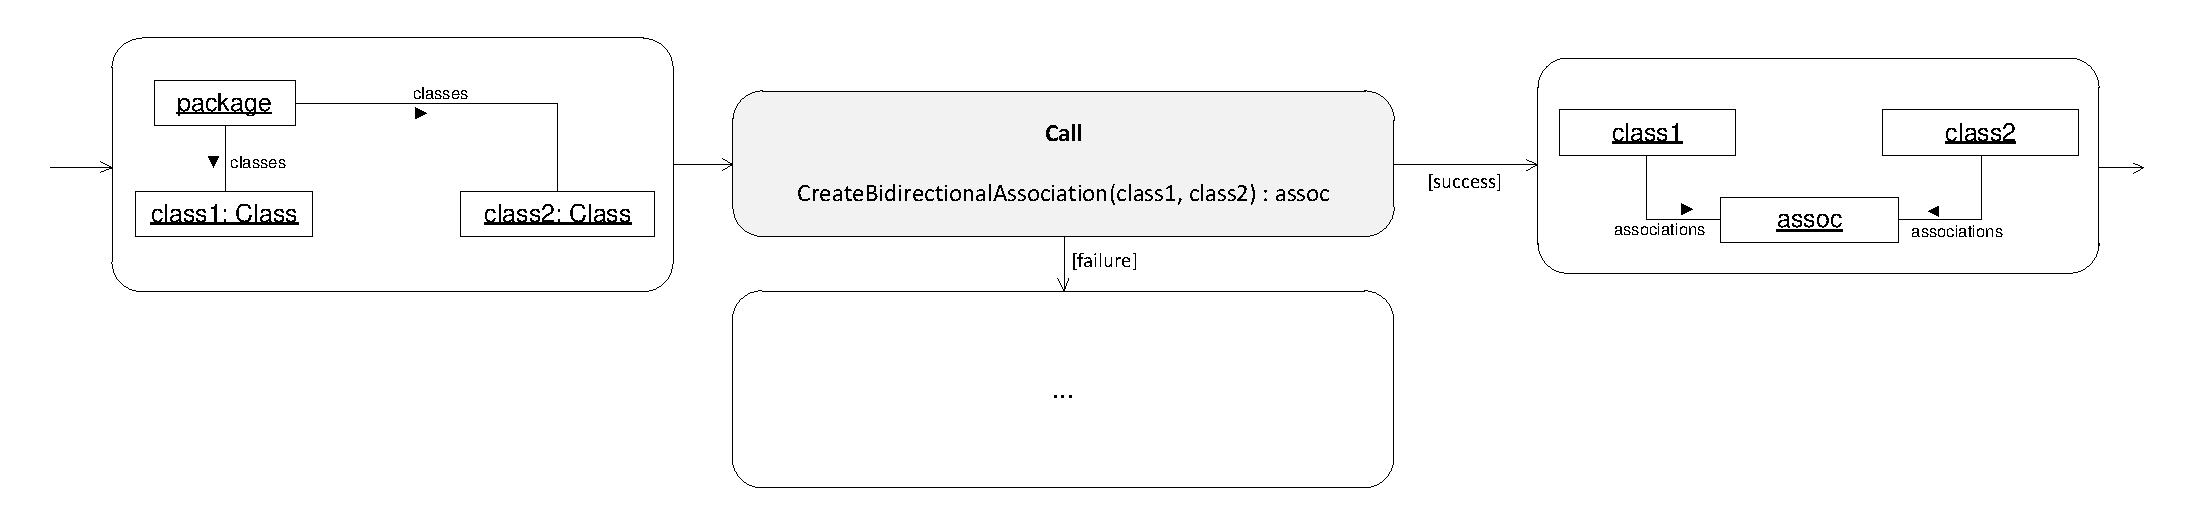
\includegraphics[width=\textwidth]{figures/StoryDiagramCall}
  \caption{Example of a story diagram call}
  \label{fig:call}
\end{center}
\end{figure}

The first story pattern in Figure~\ref{fig:call}, shows the bound object variable \fe{package}. Two new object variables \fe{class1} and \fe{class2} are bound in that pattern. The next node with the grey background is a story diagram call which is also signified by its label. Beneath the label, the name of the called story diagram is given, in this case \fe{CreateBidirectionalAssociation}. Assume that the called story diagram has two in parameters of the type \fe{Class} and one out parameter of the type \fe{Association}. The two classes that were bound in the first story pattern, \fe{class1} and \fe{class2} are passed to the call as arguments.
The result of the call is bound to the object variable \fe{assoc}. The type of this variable is determined by the out parameter type, i.e., in this case the type Association.

If a story diagram has no out parameters, the colon and the out parameters names after the parentheses are omitted (see Figure \ref{fig:SDRemoveInterfaceViolation} for an example).

%Issues for future versions:
% method calls
% polymorphic calls

\subsubsection{Exception Handling (maybe not in Ver. 0.1)}